\documentclass[journal,12pt,twocolumn]{IEEEtran}
%

\usepackage{setspace}
\usepackage{gensymb}
\singlespacing
\usepackage{hyperref}
\usepackage{amsmath}
\usepackage{amsthm}
\usepackage{txfonts}
\usepackage{cite}
\usepackage{enumitem}
\usepackage{mathtools}
\usepackage{listings}
    \usepackage{color}                                            %%
    \usepackage{array}                                            %%
    \usepackage{longtable}                                        %%
    \usepackage{calc}                                             %%
    \usepackage{multirow}                                         %%
    \usepackage{hhline}                                           %%
    \usepackage{ifthen}                                           %%
  %optionally (for landscape tables embedded in another document): %%
    \usepackage{lscape}     
\usepackage{multicol}
\usepackage{chngcntr}
\renewcommand\thesection{\arabic{section}}
\renewcommand\thesubsection{\thesection.\arabic{subsection}}
\renewcommand\thesubsubsection{\thesubsection.\arabic{subsubsection}}

% correct bad hyphenation here
\hyphenation{op-tical net-works semi-conduc-tor}
\def\inputGnumericTable{}                                 %%

\lstset{
%language=C,
frame=single, 
breaklines=true,
columns=fullflexible
}

\begin{document}
%


\newtheorem{theorem}{Theorem}[section]
\newtheorem{problem}{Problem}
\newtheorem{proposition}{Proposition}[section]
\newtheorem{lemma}{Lemma}[section]
\newtheorem{corollary}[theorem]{Corollary}
\newtheorem{example}{Example}[section]
\newtheorem{definition}[problem]{Definition}
\newcommand{\BEQA}{\begin{eqnarray}}
\newcommand{\EEQA}{\end{eqnarray}}
\newcommand{\define}{\stackrel{\triangle}{=}}
\bibliographystyle{IEEEtran}
\providecommand{\mbf}{\mathbf}
\providecommand{\pr}[1]{\ensuremath{\Pr\left(#1\right)}}
\providecommand{\qfunc}[1]{\ensuremath{Q\left(#1\right)}}
\providecommand{\sbrak}[1]{\ensuremath{{}\left[#1\right]}}
\providecommand{\lsbrak}[1]{\ensuremath{{}\left[#1\right.}}
\providecommand{\rsbrak}[1]{\ensuremath{{}\left.#1\right]}}
\providecommand{\brak}[1]{\ensuremath{\left(#1\right)}}
\providecommand{\lbrak}[1]{\ensuremath{\left(#1\right.}}
\providecommand{\rbrak}[1]{\ensuremath{\left.#1\right)}}
\providecommand{\cbrak}[1]{\ensuremath{\left\{#1\right\}}}
\providecommand{\lcbrak}[1]{\ensuremath{\left\{#1\right.}}
\providecommand{\rcbrak}[1]{\ensuremath{\left.#1\right\}}}
\theoremstyle{remark}
\newtheorem{rem}{Remark}
\newcommand{\sgn}{\mathop{\mathrm{sgn}}}
\providecommand{\abs}[1]{\lvert#1\rvert}
\providecommand{\res}[1]{\Res\displaylimits_{#1}} 
\providecommand{\norm}[1]{\lVert#1\rVert}
\providecommand{\mtx}[1]{\mathbf{#1}}
% \providecommand{\mean}[1]{E\left[ #1 \right]}
\providecommand{\fourier}{\overset{\mathcal{F}}{ \rightleftharpoons}}
\providecommand{\system}{\overset{\mathcal{H}}{ \longleftrightarrow}}
\newcommand{\solution}{\noindent \textbf{Solution: }}
\newcommand{\cosec}{\,\text{cosec}\,}
\providecommand{\dec}[2]{\ensuremath{\overset{#1}{\underset{#2}{\gtrless}}}}
\newcommand{\myvec}[1]{\ensuremath{\begin{pmatrix}#1\end{pmatrix}}}
\newcommand{\cmyvec}[1]{\ensuremath{\begin{pmatrix*}[c]#1\end{pmatrix*}}}
\newcommand{\mydet}[1]{\ensuremath{\begin{vmatrix}#1\end{vmatrix}}}
\newcommand{\proj}[2]{\textbf{proj}_{\vec{#1}}\vec{#2}}
\newcommand{\RNum}[1]{\uppercase\expandafter{\romannumeral #1\relax}}
\let\StandardTheFigure\thefigure
\let\vec\mathbf
\title{
\LARGE SM5083\\
    \LARGE Assignment Number 02 \\[0.5em]
    
    \large Jaydeep singh chouhan\par
    \large   SM21MTECH12005  \par
}
\maketitle
\renewcommand{\thefigure}{\theenumi}
\renewcommand{\thetable}{\theenumi}
\section{ Chapter \RNum{3}  miscellaneous example \RNum{4} Q.1}
\renewcommand{\theequation}{\theenumi}
\begin{enumerate}[label=\thesection.\arabic*.,ref=\thesection.\theenumi]
\numberwithin{equation}{enumi}
\item show that the equation of line joining $(r_1,\theta_1),(r_2,\theta_2)$
is $$ \frac{1}{r} \sin{(\theta_1-\theta_2)}=\frac{1}{r_1} \sin{(\theta-\theta_2)}+\frac{1}{r_2} \sin{(\theta-\theta_1)}$$\\
\solution
The python code is available at
 \begin{lstlisting}
https://github.com/jaydeep-singh-chouhan/line-/blob/main/%20line.ipynb
\end{lstlisting}
let \begin{align}
    \begin{vmatrix}
    r\cos\theta&r_1\cos\theta_1&r_2\cos\theta_2\\
    r\sin\theta&r_1\sin\theta_1&r_2\sin\theta_2\\
    1&1&1
    \end{vmatrix}
    =0
\end{align}

\begin{align}\nonumber
 r_1r_2(\cos\theta_1\sin\theta_2-\sin\theta_1\cos\theta_2)\\\nonumber
 -rr_2(\cos\theta\sin\theta_2-\sin\theta\cos\theta_2)\\\nonumber
 +rr_1(\cos\theta\sin\theta_1-\sin\theta\cos\theta_1=0\\
\end{align}
\begin{align}\nonumber
-r_1r_2\sin(\theta_1-\theta_2)+rr_2\sin(\theta-\theta_2)\\\nonumber
-rr_1\sin(\theta-\theta_1)=0\\
\end{align}
now rearranging the equation 1.1.3 we get 
\begin{align}
\frac{1}{r} \sin{(\theta_1-\theta_2)}=\frac{1}{r_1} \sin{(\theta-\theta_2)}+\frac{1}{r_2} \sin{(\theta-\theta_1)}
 \end{align}
 let us assume  any r1 , r2 , $\theta_1$ , $\theta_2$\\
 \begin{align}
     r_1=3\\
     r_2=4\\
     \theta_1=\frac{\pi}{3}\\
     \theta_2=\frac{\pi}{6}\\\nonumber
 \end{align}
 Take any point of the line \\
 let it be A\\
\begin{align}
A=(3.464,2)\\
\vec{A}=\myvec{3.464\\2}\\
r=\norm{\vec{A}}=3.999\\
\theta=\arctan\frac{2}{3.464}=30\\\nonumber
\end{align}

 
 \begin{figure}[!ht]
	\centering
	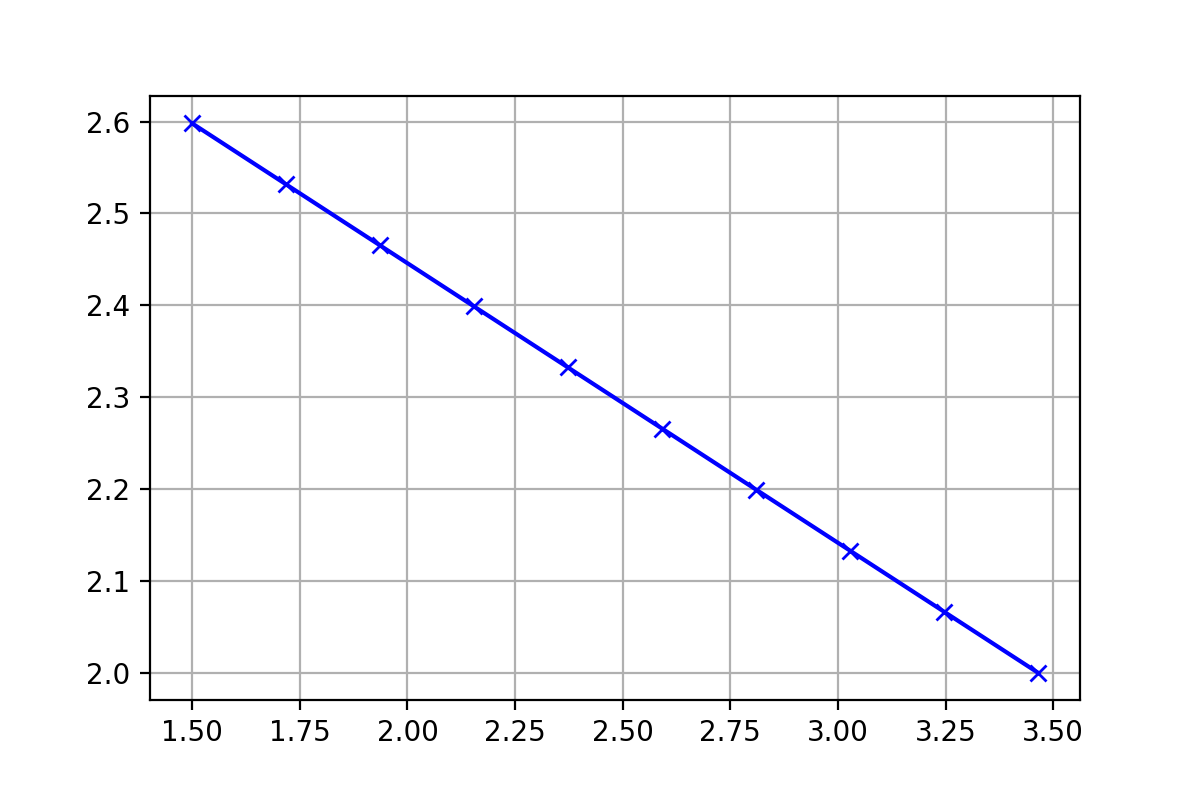
\includegraphics[width=\columnwidth]{line.png}
	\caption{line generated}
	\label{fig:line}
\end{figure}

\end{enumerate}
\end{document}
